\section{Ejercicio 1: Solución exacta}

  % \begin{figure}[ht]
  %   \begin{center}
  %     \includegraphics[width=0.5\columnwidth]{imagenes/pacman.png}
  %     \caption{Perdidos y con poca fuerza}
  %   \end{center}
  % \end{figure}

    % 1. Describir detalladamente el problema a resolver dando ejemplos del mismo y sus soluciones.
    \subsection{Descripción del problema y solución propuesta}
        En este primer acercamiento, se pidió realizar un algoritmo exacto que resuelva el problema en cuestión. El mísmo debía contener podas y estrategias que permitan mejorar el tiempo de ejecución pero que aseguren devolver la solución correcta (en caso de haber).

        Una solución existe cuando se pueden conquistar todos los gimnasios y además es exacta cuando se conquistan todos ellos recorriendo la menor distancia posible.

    % 2. Explicar de forma clara, sencilla, estructurada y concisa, las ideas desarrolladas para la resolución del problema. Utilizar pseudocódigo y lenguaje coloquial (no código fuente). Justificar por qué el procedimiento resuelve efectivamente el problema.
        Dado que nuestro problema es una instancia del TSP mencionado en la introducción, resolvimos encontrar la solución exacta utilizando la técnica de \textit{backtracking}. Esto es probar todas las soluciones posibles descartando la mayor cantidad que no sean correctas a la vez mediante el uso de \textit{podas}, para así obtener lo más rápido posible la solución correcta. Cada solución se  construye de manera tal que en cada iteración se agrega parte de una posible solución. En este caso, lo que se hace es recorrer el grafo desde cada nodo probando todos los caminos posibles, es decir, partiendo de cada gimnasio o pokeparada, conquistar todos los gimnasios pociones todas las formas posibles sin pasar dos veces por el mismo lugar. Las podas utilizadas fueron las siguientes:
            \begin{itemize}
                \item{Verificar al principio que dado pociones($g$) el número de pociones para un gimnasio $g$, \newline $\sum_{g \in Gimnasios} pociones(g) \leq m*3$ con $m$ cantidad de pokeparadas no recorridas}
                \item{Verificar al principio que $\forall g \in Gimnasios$ ($k \geq$ pociones($g$)) con $k$ el tamaño de la mochila}
                \item{Chequear que en todo momento el recorrido que se está llevando a cabo tiene distancia menor o igual a la solución actual si es que ya se encontró una}
                \item{No pasar por pokeparadas si la mochila está llena}
            \end{itemize}

        En cada iteración, se visita un nuevo punto (gimnasio o pokeparada), agregando la distancia correspondiente a la posible solución.


        \subsection{Detalles implementativos}
            Para modelar las pokeparadas y gimnasios, implementamos la clase \textit{Estacion}, la cual consiste en: un booleano para decidir si es gimasio o pokeparada, un entero que indica la cantidad de pociones y un id único para cada estación (el cual se da segun el número de linea de la entrada). Para determinar el valor de pociones, en el caso de las pokeparadas es simplemente 3 ya que es la cantidad que entrega cada una, mientras que en el caso de los gimnasios es 0 menos el número de pociones necesarias para ganarlo, que se pasa en el input. Esto es justamente porque los gimnasios consumen pociones de la mochila.

            Para trabajar las distancias entre cada punto, construímos una matriz formada con vectores de vectores, en los que cada índice es el ID del primer nodo con el ID del segundo y para cada posicion $(i,v)$ se encuentra la distancia entre los nodos i y j, la cual se calcula mediante pitágoras.

            La función principal de Backtracking recibe como parámetros un vector de Estaciones, que consiste en todas las estaciones aún no visitadas ($estaciones$), la matriz de distancias ($distancias$), el tamaño de la mochila ($k$), un vector de Estaciones visitadas ($visitados$), la cantidad de pociones actuales ($potasActuales$) y una tupla de $double$, $int$ y vector de $int$ que representa la solución actual ($solucion$). La misma realiza la lógica descripta en el siguiente pseudocódigo:

            \begin{codesnippet}
            \begin{verbatim}
BT_capturar_gimnasios(lista<Estacion> estaciones, lista< lista<double> > distancias,
entero k, lista<Estacion> visitados, entero potasActuales,
tupla<double,entero,lista<IDs> > soluciones):
  si es solucion(estaciones):
    distancia = distancia_acumulada(visitados,distancias)
    lista<IDs> camino                                   //(un ID es un numero entero)
    para i = 0 hasta tamaño(visitados):
      agregar id(visitados[i]) a camino
    fin para
    soluciones = tupla(distancia, tamaño(visitados), camino)
  si no:
    para i = 0 hasta tamaño(estaciones):
      nueva_distancia = 0
      si tamaño(visitados) > 0:
        id_ultimo_visitado = id(ultimo(visitados))
        proxima_distancia = distancias[id_ultimo_visitado][id(estaciones[i])]
        nueva_distancia = proxima_distancia + distancia_acumulada(visitados,distancias)
      fin si
      si (soluciones[0] >= 0 y nueva_distancia < soluciones[0] ó soluciones[0] < 0):
        si (puede_ganar_gimnasio(estaciones[i],potasActuales) ó
            puede_recibir_potas(estaciones[i],potasActuales,k)):
          agregar estaciones[i] a visitados
          si (esGimnasio(estaciones[i]) ó potasActuales + 3 <= k)
            potasActuales = potasActuales + estaciones[i].potas
          si no
            potasActuales = k
          fin si
          borrar elemento con índice i de estaciones
          BT_capturar_gimnasios(estaciones,distancias,k,visitados,potasActuales,soluciones)
          ultimaEstacion = ultimo(visitados)
          eliminar el último de visitados
          insertar ultimaEstacion en posición i de estaciones
        fin si
      fin si
    fin para
  fin si
  devolver soluciones
fin BT_capturar_gimnasios
            \end{verbatim}
            \end{codesnippet}

            En cada iteración de la función, se chequea si el estado actual de los parametros es una solución al problema. Para esto, se revisa todo el vector de estaciones en búsqueda de algúna Estación que sea gimnasio. Si no hay, entonces efectivamente es una solución y se construye la tupla con lo que devuelve el algoritmo para luego imprimir el output correspondiente. Caso contrario, se recorre todo el vector de estaciones para chequear todos los posibles lugares a los que se puede ir desde la ubicación actual e ir a todos ellos.

            Para decidir si podemos ir o no a una estación chequeamos la cantidad de pociones actuales que se tienen junto con el tamaño de la mochila y las pociones de la estación a la que se desea ir. Si es un gimnasio, analizamos si $pociones + pociones(gimnasio) > 0$. Dado que el gimnasio tiene la cantidad de pociones en negativo (como mencionamos anteriormente), si esta suma deciende de 0 quiere decir que las pociones que tenemos en la mochila no son suficientes para conquistar ese gimnasio, por lo que no tendría sentido ir ya que esto solamente aumentaría la distancia recorrida (y esto último ocurre porque como todas las estaciones están conectadas,  $\forall v,w,r \in Estaciones : distancia(v,w) \leq distancia(v,r) + distancia(r,w)$). Si es una pokeparada, observamos si $pociones = k$ con $k$ tamaño de la mochila. La razón es que cada pokeparada otorga 3 pociones pero si la mochila se llena entonces se descartan las excedentes. En particular, si la mochila esta totalmente llena, se descartan todas las pociones de esa pokeparada; y teniendo en cuenta lo dicho recientemente, si hay solución debería existir otra estación tal que se pueda visitar sin agregar innecesariamente distancia recorrida a la solución actual.

            Antes de entrar en la función descripta, se realizan dos chequeos (las podas). Primero, que no exista un gimnasio cuya cantidad de pociones sea mayor al tamaño de la mochila, ya que si esto ocurriera, incluso pasando por todas las pokeparadas posibles nunca alcanzaríamos la cantidad necesaria para conquistar ese gimnasio. Un ejemplo puede ser 2 pokeparadas, 1 gimnasio que necesita 10 pociones y tamaño de mochila 9. En segundo lugar, que la suma total de pociones necesarias para conquistar a cada gimnasio sea menor o igual a la cantidad de $pokeparadas*3$. Esto se hace para descartar los casos en los que incluso teniendo el tamaño de mochila suficiente para guardar todas las pociones de todas las pokeparadas, las mismas no alcancen para conquistar todos los gimnasios. Un caso ejemplo sería 1 pokeparada, 2 gimnasios que necesitan 3 pociones y tamaño de mochila 3.


    % 3. Deducir una cota de complejidad temporal del algoritmo propuesto y justificar por qué el algoritmo cumple la cota dada. Utilizar el modelo uniforme.
    \subsection{Complejidad teórica}

      La primeras dos podas, que son los chequeos que se realizan antes de llamar a la función principal, consisten en recorrer el vector de Estaciones sumando y restando valores de pociones, por lo que es $O(n+m)$ temporal y $O(1)$ espacial ya que solo crean 2 variables enteras.

      El algoritmo principal lo primero que hace es chequear si el estado actual de los parámentros, como se dijo anteriormente, corresponden a una solución del problema. Este análisis toma $O(n+m)$ temporal y $O(1)$ espacial ya que solo es recorrer el vector de Estaciones para chequear si existen gimnasios no visitados. Si es solución, se obtiene la distancia acumulada, que toma $O(n+m)$ ya que es solamente recorrer el vector de visitados (y por lo tanto $O(1)$ espacial) y luego se recorre nuevamente el mismo vector para obtener el camino que se realizó, costando $O(n+m)$ temporal y $O(1)$ espacial.
      Si no es solución se recorren todas las estaciones del vector estaciones (que tomará $O(n+m)$) realizando los siguientes pasos para cada una: Si la cantidad de Estaciones visitadas es mayor a 0 (cosa que no ocurrirá solamente en la primera iteración) se obtiene la distancia acumulada más la proxima distancia a sumar, que como dijimos en el párrafo anterior cuesta $O(n+m)$. Luego, si esa distancia es menor que la distancia de la solución encontrada hasta ahora (si la hubiera) y puede ir a conquistar el gimnasio (si el la próxima posición lo es) o la cantidad de pociones es menor al tamaño de la mochila (y la próxima posición es una pokeparada), se agrega al vector de visitados la próxima estación ($O(1)$ amortizado), se actualiza el valor de pociones ($O(1)$), se elimina la estación del vector estaciones ($O(n+m)$), se llama a la función recursiva (luego explicado) y por último se vuelve al estado original los vectores de visitados y estaciones ($O(n+m)$ temporal y $O(1)$ espacial cada uno).
      El llamado a la función recursiva hace que para cada Estación del vector de estaciones se recorran todas las demás en búsqueda de una solución, por lo que una iteración tomaría $O(n+m)$ temporal y como todos los vectores se pasan siempre por referencia, solo tomaría $O(1)$ espacial (sin contar el overhead en el $stack$ de llamadas recursivas). Luego, como en cada iteración se realiza todo lo mencionado y en total son ($n+m$) iteraciones, en total costará
      \[
        O(\prod_{i=0}^{n+m} i)*O(n+m)
      \]
      \[
        \in O((n+m)! * (n+m))
      \]

      Por lo que el algoritmo tiene complejidad temporal $O((n+m)! * (n+m))$ y espacial $O((n+m)^2)$ por la matriz de distancia que se construye antes de llamar a la función principal.

    % 4. Dar un código fuente claro que implemente la solución propuesta. Se deben incluir las partes relevantes del código como apéndice del informe impreso entregado.

    % 5. Realizar una experimentación computacional para medir la performance del programa implementado. Usar un conjunto de casos de test en función de los parámetros de entrada, con instancias aleatorias e instancias particulares (de peor/mejor caso en tiempo de ejecución, por ejemplo). Presentar en forma gráfica una comparación entre los tiempos medidos y la complejidad teórica calculada y extraer conclusiones.
    \subsection{Experimentación}

      Los experimentos que realizamos para observar los tiempos de ejecución del algoritmo en función del tamaño de entrada y de las podas implementadas consistieron en el análisis de casos que contemplan:

      \begin{itemize}
        \item El comportamiento de las podas
        \item Configuraciones de valores que no están en la cota de complejidad
        \item Configuraciones de valores que sí están en la cota de complejidad, dejando fijos los demás
      \end{itemize}

      Para todos los casos, el algoritmo se ejecutó 30 veces con cada instancia para intentar tener la mayor presición posible en cuanto a tiempo de ejecución.

      \subsubsection{Experimento 1}
      En esta instancia generamos entradas que aumentaban linealmente de 1 a 10 la cantidad de pokeparadas y gimnasios, variando el tamaño de la mochila y marcando a cada gimnasio con la cantidad de pociones necesarias igual al numero de linea en el input (para el gimnasio $k$, se piden $k$ pociones). Además, las ubicaciones de cada estación se setearon cada una a distancia 1 de la anterior y de forma que para la estación $i$ la ubicación es ($i$,$i$).

      Algunos ejemplos para el input de este experimento son los siguientes:


      \begin{codesnippet}
\begin{verbatim}
8 8 36        9 9 45        10 10 55
1 1 1         1 1 1         1 1 1
2 2 2         2 2 2         2 2 2
3 3 3         3 3 3         3 3 3
4 4 4         4 4 4         4 4 4
5 5 5         5 5 5         5 5 5
6 6 6         6 6 6         6 6 6
7 7 7         7 7 7         7 7 7
8 8 8         8 8 8         8 8 8
9 9           9 9 9         9 9 9
10 10         10 10         10 10 10
11 11         11 11         11 11
12 12         12 12         12 12
13 13         13 13         13 13
14 14         14 14         14 14
15 15         15 15         15 15
16 16         16 16         16 16
              17 17         17 17
              18 18         18 18
                            19 19
                            20 20

\end{verbatim}
      \end{codesnippet}

      Las primeras 10 entradas se seteó para que el tamaño de la mochila sea $n*m$, es decir que para cada entrada, si la cantidad de gimnasios es $n$ y la de pokeparadas $m$, entonces el tamaño de la mochila es $n*m$ (eg, 3 gimnasios y 3 pokeparadas, la mochila tiene tamaño 9). Para las siguientes 10 entradas el tamaño de la mochila es $\sum_{g \in gimnasios} pociones(g)$. En las últimas 10, el tamaño se seteó como $n+m$. 
      Para este experimento, esperabamos que para las primeras 20 instancias el algoritmo tome más tiempo que para las últimas 10, ya que si el tamaño de la mochila $k \geq 3*m$ entonces se pueden guardar todas las pociones de todas las pokeparadas antes de ir a algun gimnasio, mientras que en caso contrario, habrá muchos caminos en los que primero se pasen por pokeparadas sin ir a gimnasios que no se podrían realizar porque siguiendo la poda de que si la mochila está llena no vamos a una pokeparada, la misma se llenaría mucho más rápido y esto impediría que sigamos por esos caminos.
      Aprovechamos este mismo exprimento para correrlo sin y con la poda de chequeo que el total de pociones de todos los gimnasios debe ser mayor o igual a $3*m$ para mostrar la diferencia de comportamiento.
      Los resultados de tiempo en funcion de la cantidad de estaciones según el tamaño de la mochila para el algoritmo sin la poda puede verse en el siguiente gráfico, el cual tiene además una función que sigue la cota de complejidad que es solo para dar una idea de cómo es la misma.

  \begin{figure}[H]
      \begin{center}
        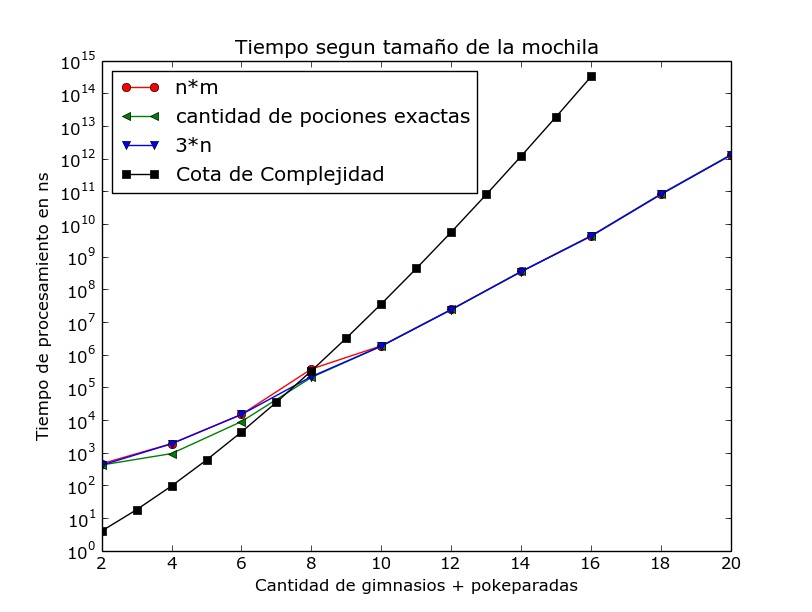
\includegraphics[width=0.7\columnwidth]{imagenes/exp1_ej1_nuevo.jpeg}
        \caption{}
      \end{center}
  \end{figure}

      Mientras que los resultados con la poda son los siguientes:

  \begin{figure}[H]
      \begin{center}
        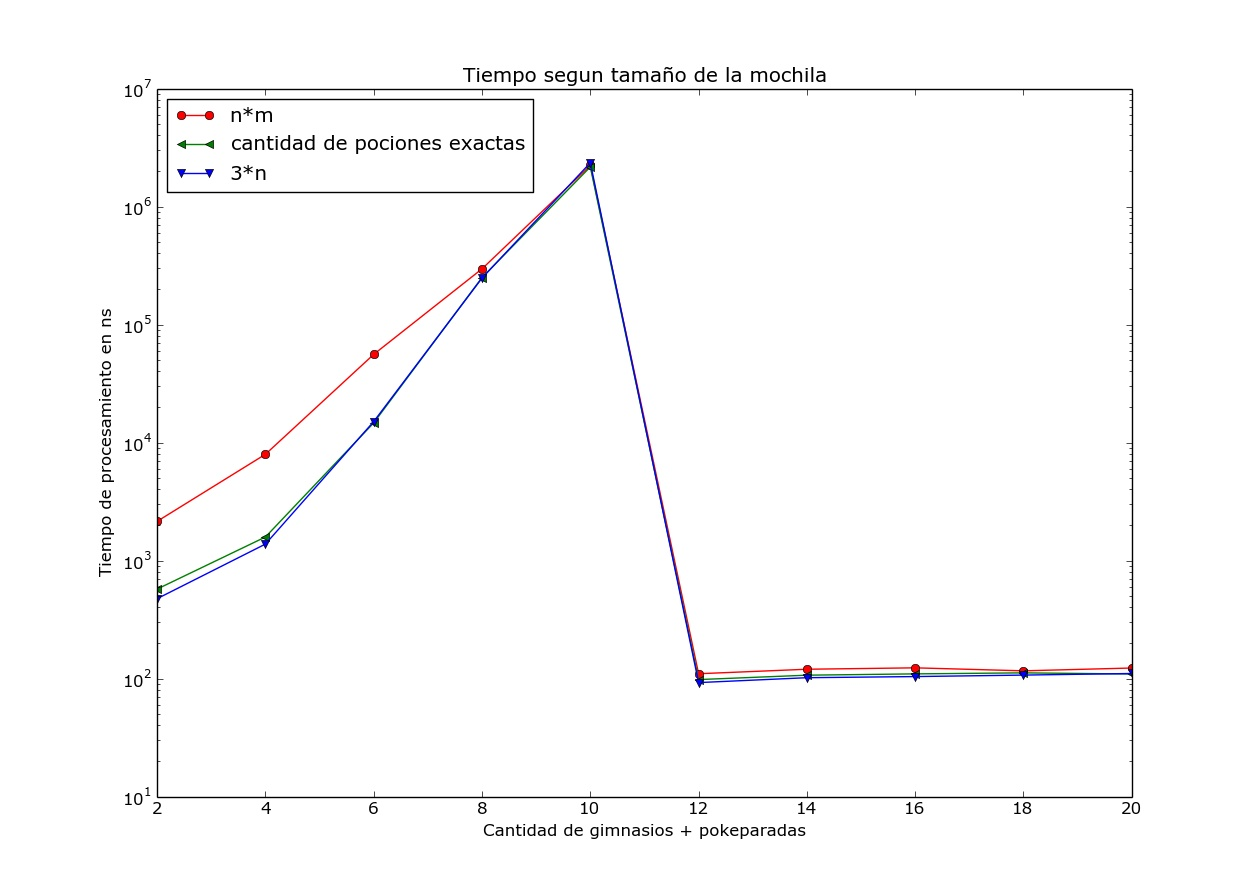
\includegraphics[width=0.7\columnwidth]{imagenes/exp1_2_ej1_nuevo.jpeg}
        \caption{}
      \end{center}
  \end{figure}

      En cuanto al primer gráfico, nos llevamos la sopresa de que las podas que cortan las posibles soluciones que sean peores que la solución actual y que aseguran no ir a una pokeparada si la mochila está llena no fueron muy útiles, pues notamos que los resultados en tiempo son muy similares en cada caso. Tanto, que en el gráfico las líneas de cada instancia están solapadas, pudiendo notarlo en los puntos marcados, que están los marcadores correspondientes a cada línea uno encima del otro.

      Respecto al segundo gráfico, notamos que a partir de las 12 estaciones (6 pokeparadas y 6 gimnasios) las podas funcionaron adecuadamente, ya que para esas instancias la cantidad de gimnasios no alcanzaba para cubrir todos los gimnasios (había entre 21 pociones necesarias con 6 pokeparadas hasta 110 pociones necesarias con 10 pokeparadas). Tambien observamos que los tiempos para cada tamaño de mochila no variaba mucho de los otros, por lo que decidimos hacer otro experimento en el que se observe el tiempo de ejecución cuando lo que varía es la cantidad de pociones necesarias para cada gimnasio.

      De ambos resultados obtuvimos la información necesaria para notar que para las instancias que tienen solución, el tiempo de ejecución respecto del tamaño de la entrada crece con una forma similar a la cota de complejidad. También concluímos que las podas implementadas sirven son de mucha utilidad en instancias no necesariamente grandes (con 12 estaciones recortó mucho el tiempo de ejecución).

    \subsubsection{Experimento 2}


      Para este experimento, como mencionamos antes, construimos 16 instancias en las que aumentamos linealmente entre 1 y 8 la cantidad de pokeparadas y gimnasios (ambas al mismo tiempo), fijamos en forma relativa a la cantidad de pokeparadas el tamaño de la mochila y colocamos a cada gimnasio un valor entre 1 y 3 pociones para las primeras 8 instancias y fijamos en 3 cada una en las 8 siguientes.
      Para este experimento esperabamos que las segundas 8 instancias tomen más tiempo que las primeras, ya que en las primeras 8 hay soluciones en las que no se pasan por todas las pokeparadas, teniendo más chances de encontrar una solución mejor y que se utilice la poda que saca los casos en los que se está contruyendo una solución peor a la mejor encontrada hasta el momento. Esto ocurre porque en dos instancias con misma cantidad de pokeparadas y gimnasios, en el segundo caso es necesario pasar por todas las pokeparadas, ya que en cada gimnasio se gastan las 3 pociones que se recolectaron en alguna pokeparada, mientras que en el primer caso hay algunos gimnasios que permiten mantener algunas pociones en lugar de gastarlas todas, permitiendo ahorrar pociones en algún gimnasio para usarlas en otro.

      Los resultados obtenidos de este experimento se plasmaron en los siguientes gráficos, los cuales tienen una línea que representa (a modo de referencia) la cota de complejidad y muestran de manera aproximada el funcionamiento para entre 2 y 6 estaciones (el primero) y entre 2 y 16 estaciones (el segundo):

  \begin{figure}[H]
      \minipage{0.5\textwidth}
      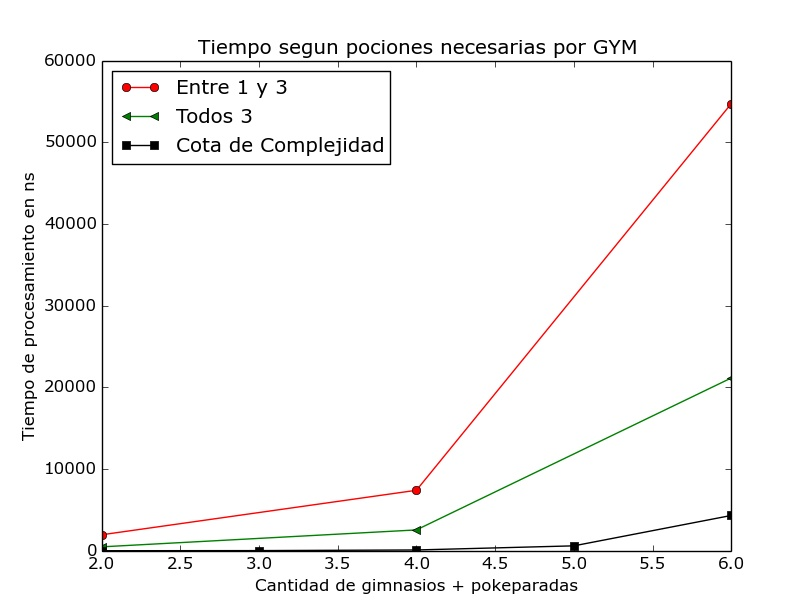
\includegraphics[width=\linewidth]{imagenes/exp2_ej1_corto.jpeg}
      \caption{2 a 6 estaciones}
      \endminipage\hfill
      \minipage{0.5\textwidth}%
      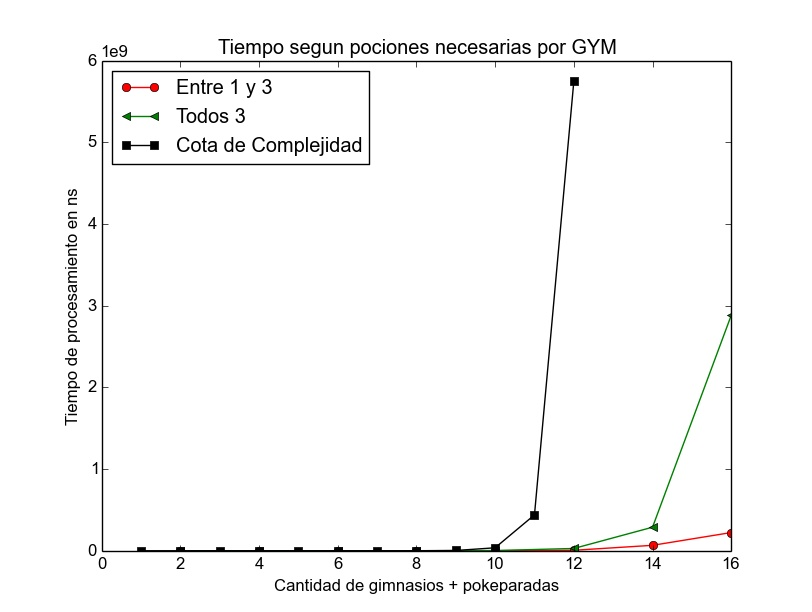
\includegraphics[width=\linewidth]{imagenes/exp2_ej1.jpeg}
      \caption{2 a 16 estaciones}
      \endminipage
  \end{figure}

      Observamos que, como esperabamos, a igual tamaño de entrada, las instancias que necesitan menor cantidad de pociones por gimnasio toman menos tiempo que las instancias que necesitan 3 o más posiones por gimnasio. Esto muestra que nuestra hipótesis funciona para los resultados de este experimento, por lo que concluímos que la poda de eliminar ramas en las que se construye una solución peor que la mejor hallada hasta el momento también resulta de utilidad cuando hay mayor cantidad de soluciones posibles. 

      Tomando los datos de los experimentos 1 y 2, pudimos notar que a pesar de que hay ciertos valores que no aparecen en la cota de complejidad, los mismos pueden cambiar el tiempo de ejecución del algoritmo, sin embargo estos cambios ocurren en gran parte gracias a las podas que sí dependen de estos valores, por lo que teóricamente la cota de complejidad esta bien planteada pero en la práctica la número de operaciones (y por lo tanto, el tiempo de ejecución) puede ser mucho menor.

    \subsubsection{Experimento 3}

      En este último experimento quisimos observar el tiempo de ejecución del algoritmo cuando varía la cantidad de pokeparadas. Para eso, creamos 20 instancias en las que se fija la cantidad de gimnasios (en 4 para las primeras 10 y 5 para las últimas), se setea un tamaño fijo para la mochila suficiente para que se puedan guardar todas las pociones al mismo tiempo  (100 en este caso) y aumentamos linealmente la cantidad de pokeparadas entre 1 y 10.
      Habiendo realizado el análisis de los experimentos anteriores y teniendo en cuenta el marco teórico de este ejercicio, propusimos como hipótesis que el tiempo de ejecución aumentaría de acuerdo a la cantidad de estaciones totales, es decir, para las primeras 10 instancias el tiempo de ejecución será menor que para las últimas 10 y además para cada instancia dentro de esas 10, la siguiente tomaría más tiempo que la anterior, ya que se agrega una pokeparada cada vez.
      El gráfico con los resultados es el siguiente:

\begin{figure}[H]
    \begin{center}
      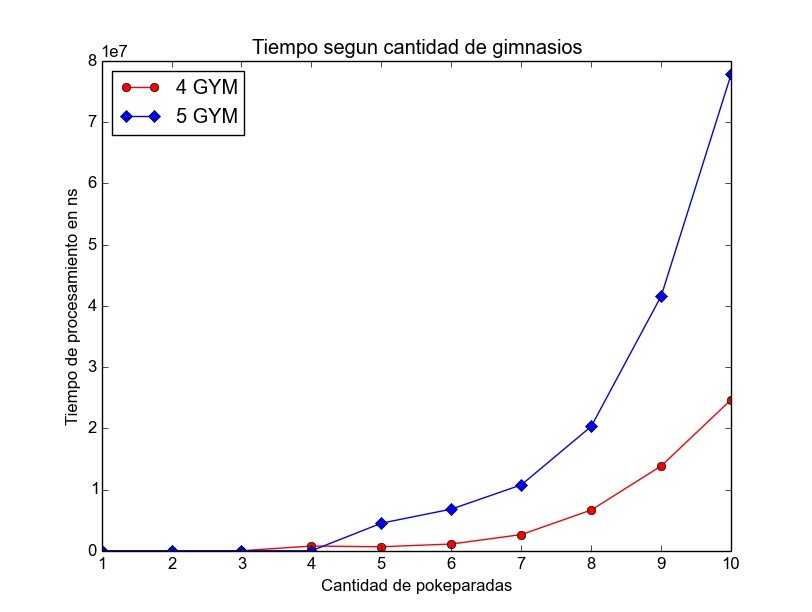
\includegraphics[width=0.7\columnwidth]{imagenes/exp4_ej1.jpeg}
      \caption{}
    \end{center}
\end{figure}

      Confirmando nuestra hipótesis, el tiempo de ejecución aumentó en cada instancia y los casos con 5 gimnasios tomaron más tiempo que los de 4. 
      Lo que sí nos llamó la atención fue que las líneas de los graficos no tienen una forma muy similar a la de la cota de complejidad, pero por lo dicho anteriormente, esto puede deberse a que gracias a las podas los tiempos de ejecución pueden ser mucho menores que lo que la teoría puede asegurar.
